\documentclass[]{book}

\usepackage{import}
\usepackage{preamble}

\begin{document}

\noindent BECA / Huson / 11.2 Algebra II \hspace{2in} Name:\\*
14 December 2017
\begin{center}
{\Large Test: Linear functions and graphing}\\
\textit{Show your work. For graphs, use a pencil and straight edge.}
\end{center}

%\vspace{0.2 cm}


\subsection*{Simplify expressions}

Simplify by collecting like terms.

\begin{enumerate}

\item $-2x^2+4x -9 +3x^2-x+9$\\*[60pt]
\item $5(a^2-2a +3) -2(3a^2-5a-4)$\\*[60pt]

\subsection*{Solve equations}

Solve for the value of $x$.
\item   $15=x-3x$\\*[50pt]
\item   $\frac{1}{2}(3-7x)=4x$\\*[60pt]
\item   $19=\frac{2}{5}x+2.6x-8$\\*[60pt]

\newpage
\subsection*{Slope-intercept form}

What is the slope and $y$-intercept of each equation? 
\item   $y=\frac{1}{2}x-3$\\*[10pt]
\item   $4x-3y=6$\\*[40pt]


\subsection*{Parallel and perpendicular linear equations}

\item What is the equation of the line with a slope of 0.5 passing through the point $(0,-3)$?\\*[40pt]
\item What is the equation of a line parallel to $y=-3x+6$ with a $y$-intercept of 5?\\*[40pt]
\item What is the slope of a line perpendicular to the line $3x-2y=11$?\\*[50pt]

\subsection*{Function substitution}
\item Given $f(x)=4x+7$. Simplify $f(2.5)$.\\*[50pt]
\item Given $\displaystyle f(x)=-\frac{(12-4x)}{5}$. Simplify $f(-2)$.

\newpage
\subsection*{Graphing linear functions}
Use pencil for graphs. Mark at least some of the values on each axis. Label each function with its name or equation. 
\item Given the function $f(x)=-\frac{1}{3}x+1$. 
\begin{enumerate}
    \item Write down the $y$-intercept.\\*[10pt]
    \item Write down the slope of $f(x)$.\\*[10pt]
    \item Draw the function $f(x)$ on the graph below.
    \item Label the intersection of $f(x)$ with the $x$-axis as the point $P$.
    \item Mark the point $Q (-3, -2)$.
    \item A second line, $g(x)$, is parallel to $f(x)$ and passes through point $Q$. Plot $g(x)$ on the graph.
    \item What is the $y$-intercept of $g(x)$?\\*[10pt]
\end{enumerate}

\begin{figure}[!ht]
    \centering
    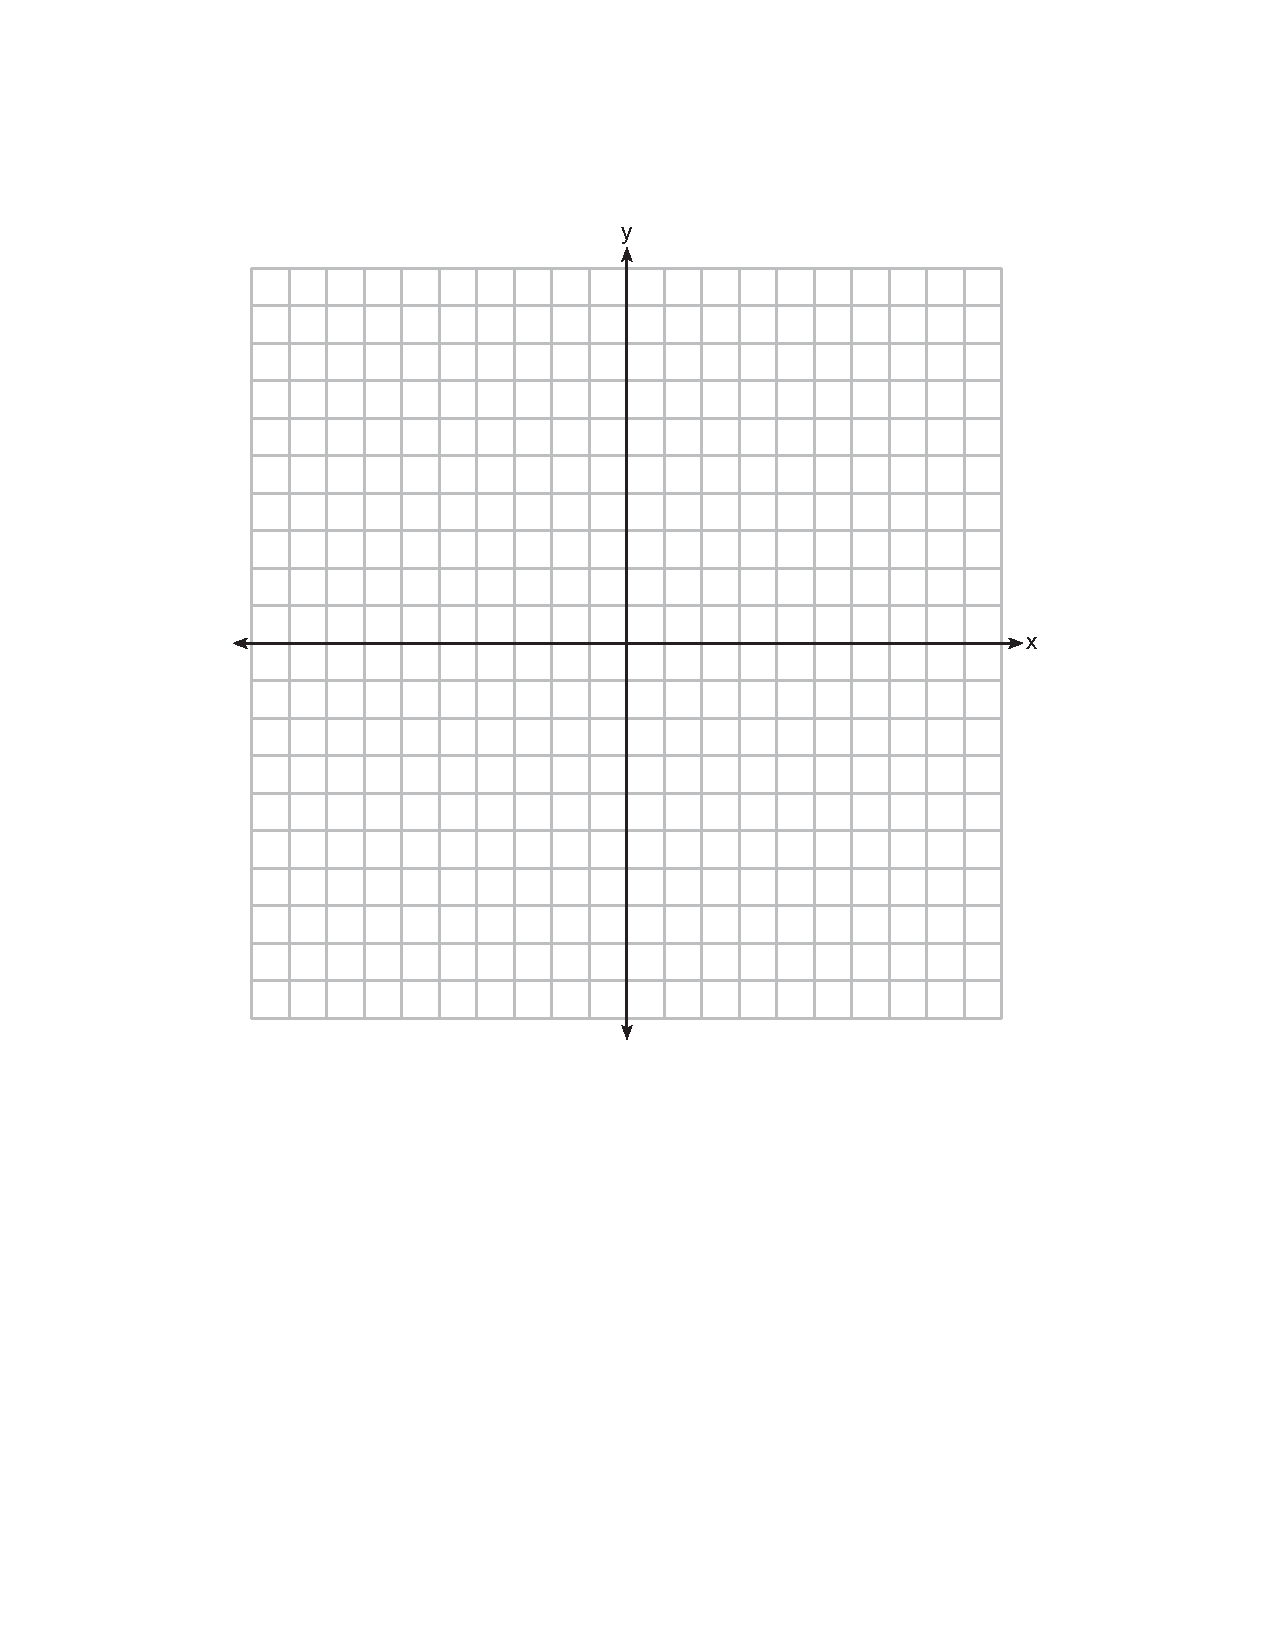
\includegraphics[width=0.75\textwidth]{regents-grid.pdf}
\end{figure}

\newpage
\item  
\begin{enumerate}
    \item Mark the point $P(6, -1)$ on the graph.
    \item The line $L_1$ has a $y$-intercept of 2 and passes through point $P$. Graph $L_1$.
    \item What is the slope of line $L_1$?\\*[20pt]
    \item What is the equation of line $L_1$?\\*[20pt]
    \item A second line, $L_2$ has the equation $2x-4y=8$. Plot $L_2$ on the graph.
    \item On the graph, mark the intersection of the two lines, the point $Q$, as an ordered pair.

\begin{figure}[!ht]
    \centering
    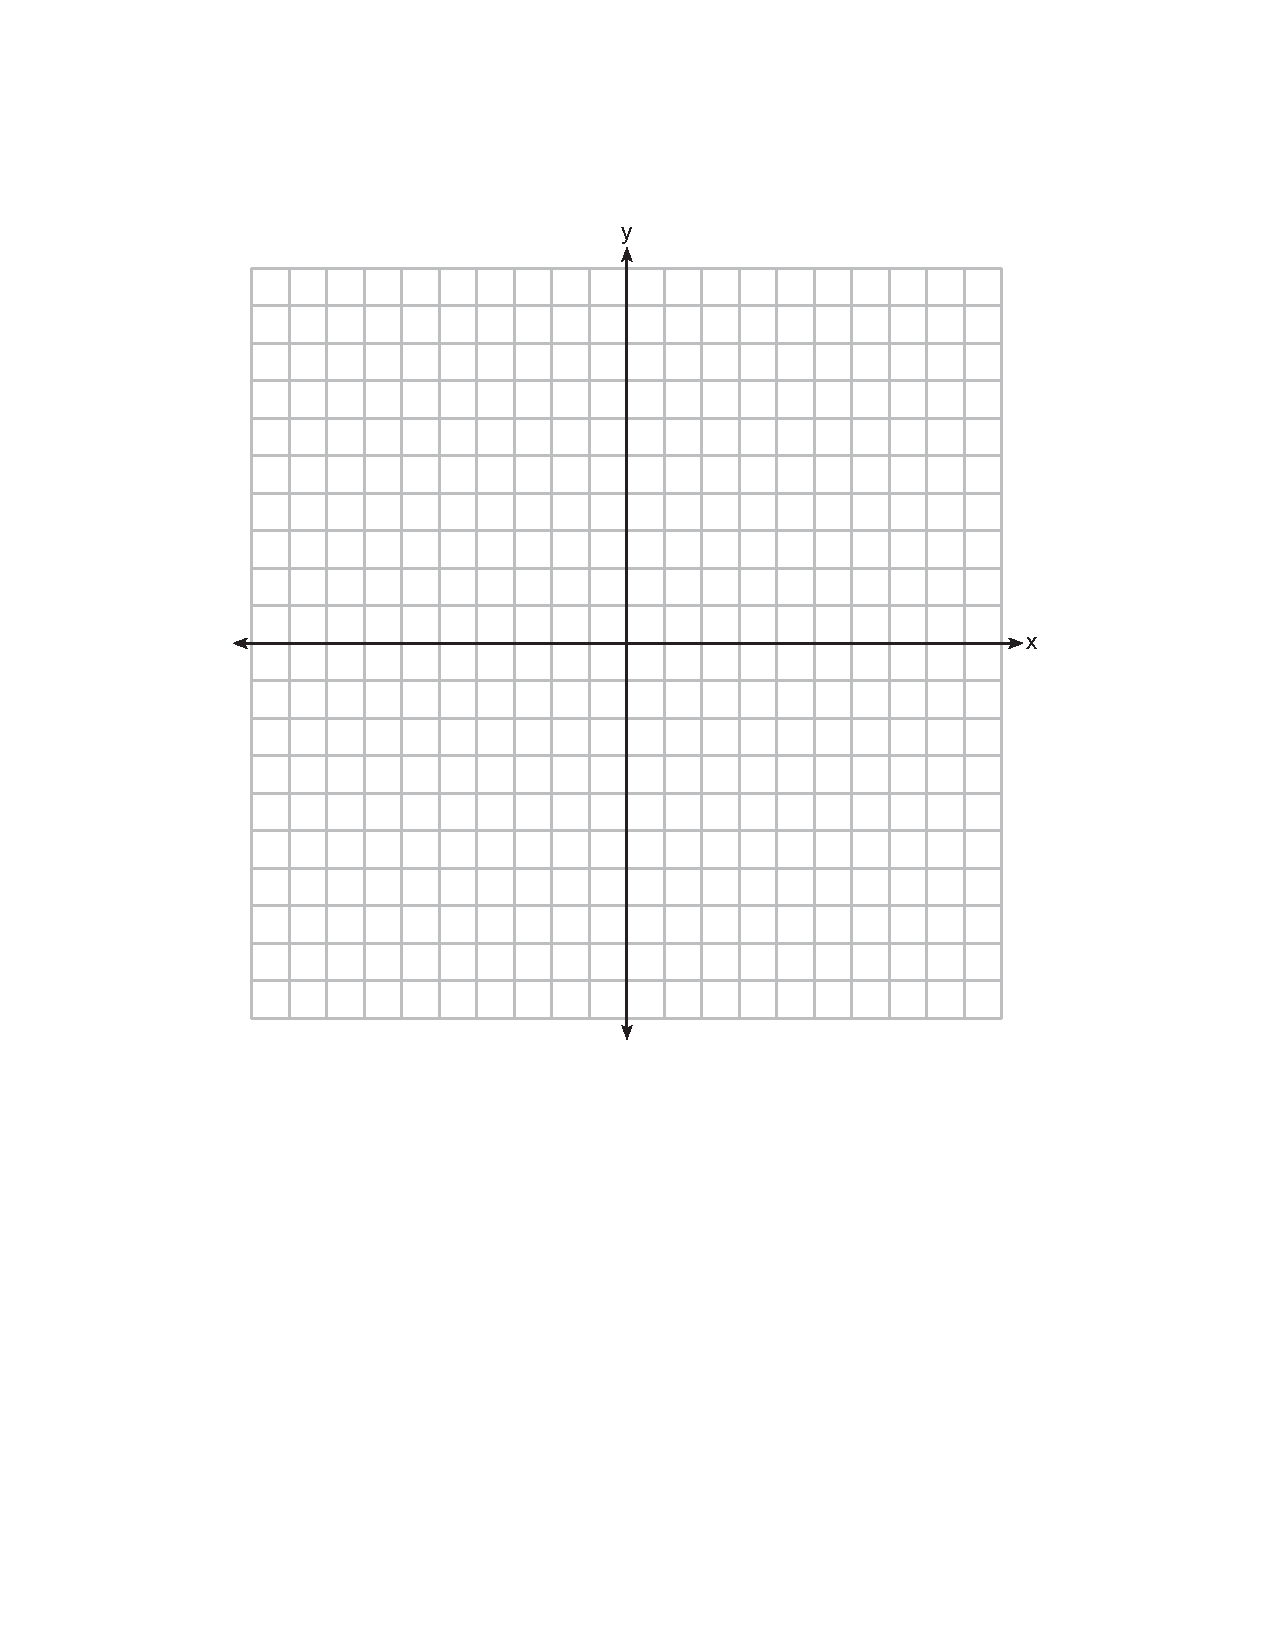
\includegraphics[width=0.65\textwidth]{regents-grid.pdf}
\end{figure}
\end{enumerate}

\item Is the expression $1+\sqrt{7}$ rational, irrational, or neither? Explain.

\newpage
\item Solve the system of equations by graphing. Select a point in the solution set and label it on the graph as ordered pair.
\[x+y>6\]
\[-3x+y \leq 2\]

\begin{figure}[!ht]
    \centering
    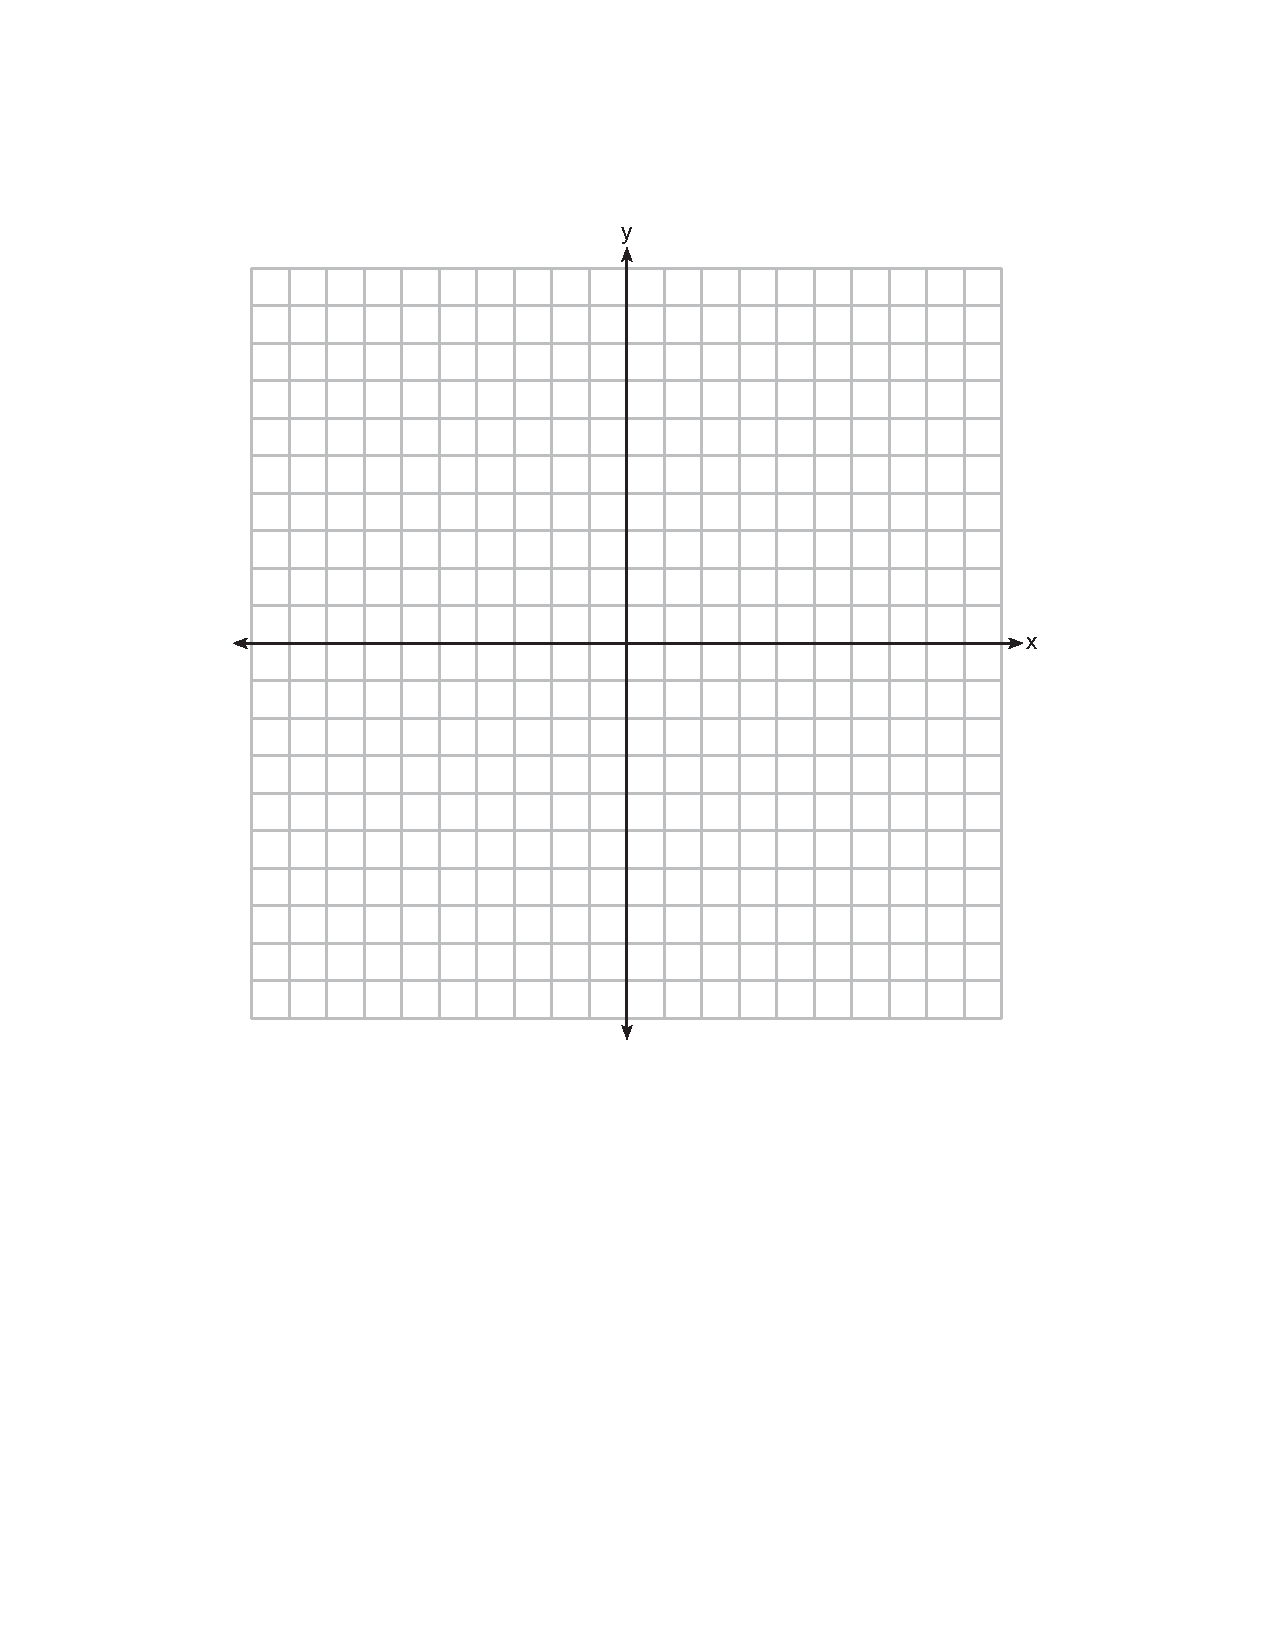
\includegraphics[width=0.65\textwidth]{regents-grid.pdf}
\end{figure}

Solve each system algebraically.
\item
$2x-4y=14$\\*
$3x-6y=21$\\*[60pt]

\item 
$2x-y=1$\\*
$3x+4y=7$

\newpage
\item Oceanside Bike Rental Shop charges a 19.50 dollar bike fee plus 6.25 dollars an hour for renting a bike. Jeffrey paid 50.75 dollars total. How many hours did he pay to have the bike checked out?\\*[140pt]

\item Four friends go bowling. The cost per person per game is \$5.75. The cost to rent shoes is \$3.50 per person. Their total cost is \$60. How many games did they play?\\*[140pt]

\item The admission fee at a small fair is \$1.50 for children and \$4.00 for adults. On a certain day, 40 people enter the fair and \$110.00 is collected. How many children and how many adults attended?

\end{enumerate}
\end{document}